\chapter{Metodologi dan Desain Sistem}
Metode yang akan digunakan pada TA ini adalah Artificial Neural Network. Data hasil analisa Demirbilek et al (2007) \cite{DemirbilekReport} akan dibagi 2. Yakni 80 persen untuk training, dan 20 persen untuk testing. Masing masing, akan disimpan ke dalam file csv. Sistem akan membaca data training langsung dari file, lalu dimasukannya sebagai input ke dalam algoritma ANN. Setelah training, sistem akan menghasilkan suatu model dengan matriks dengan attribut $W_{input}$ dan $W_{output}$ di dalamnya. Tujuannya adalah mendapatkan suatu model yang cukup baik untuk menghasilkan prediksi yang cukup akurat.

\section{Deskripsi Data}
Data yang akan digunakan dalam aplikasi neural network di TA ini adalah data hasil analisis dari eksperimen yang di lakukan oleh US Army Corps of Engineer pada Agustus - September 2006. Analisa dilakukan oleh Demirbilek et al. dan di tulis dalam laporan yang berjudul \emph{"Laboratory Study of Wind Effect on Runup over Fringing Reefs"}.

\subsection{Kondisi Eksperimen}
\label{kondisiEksperimen}

Eksperimen dibagi menjadi 3 bagian. Eksperimen pertama dilakukan hanya menggunakan variabel gelombang, dengan kecepatan angin 0. Eksperimen kedua, dilakukan hanya menggunakan variabel angin. Selanjutnya eksperimen ketiga adalah gabungan dari perubahan variable gelombang dan variabel angin.

\begin{figure}
  \begin{center}
    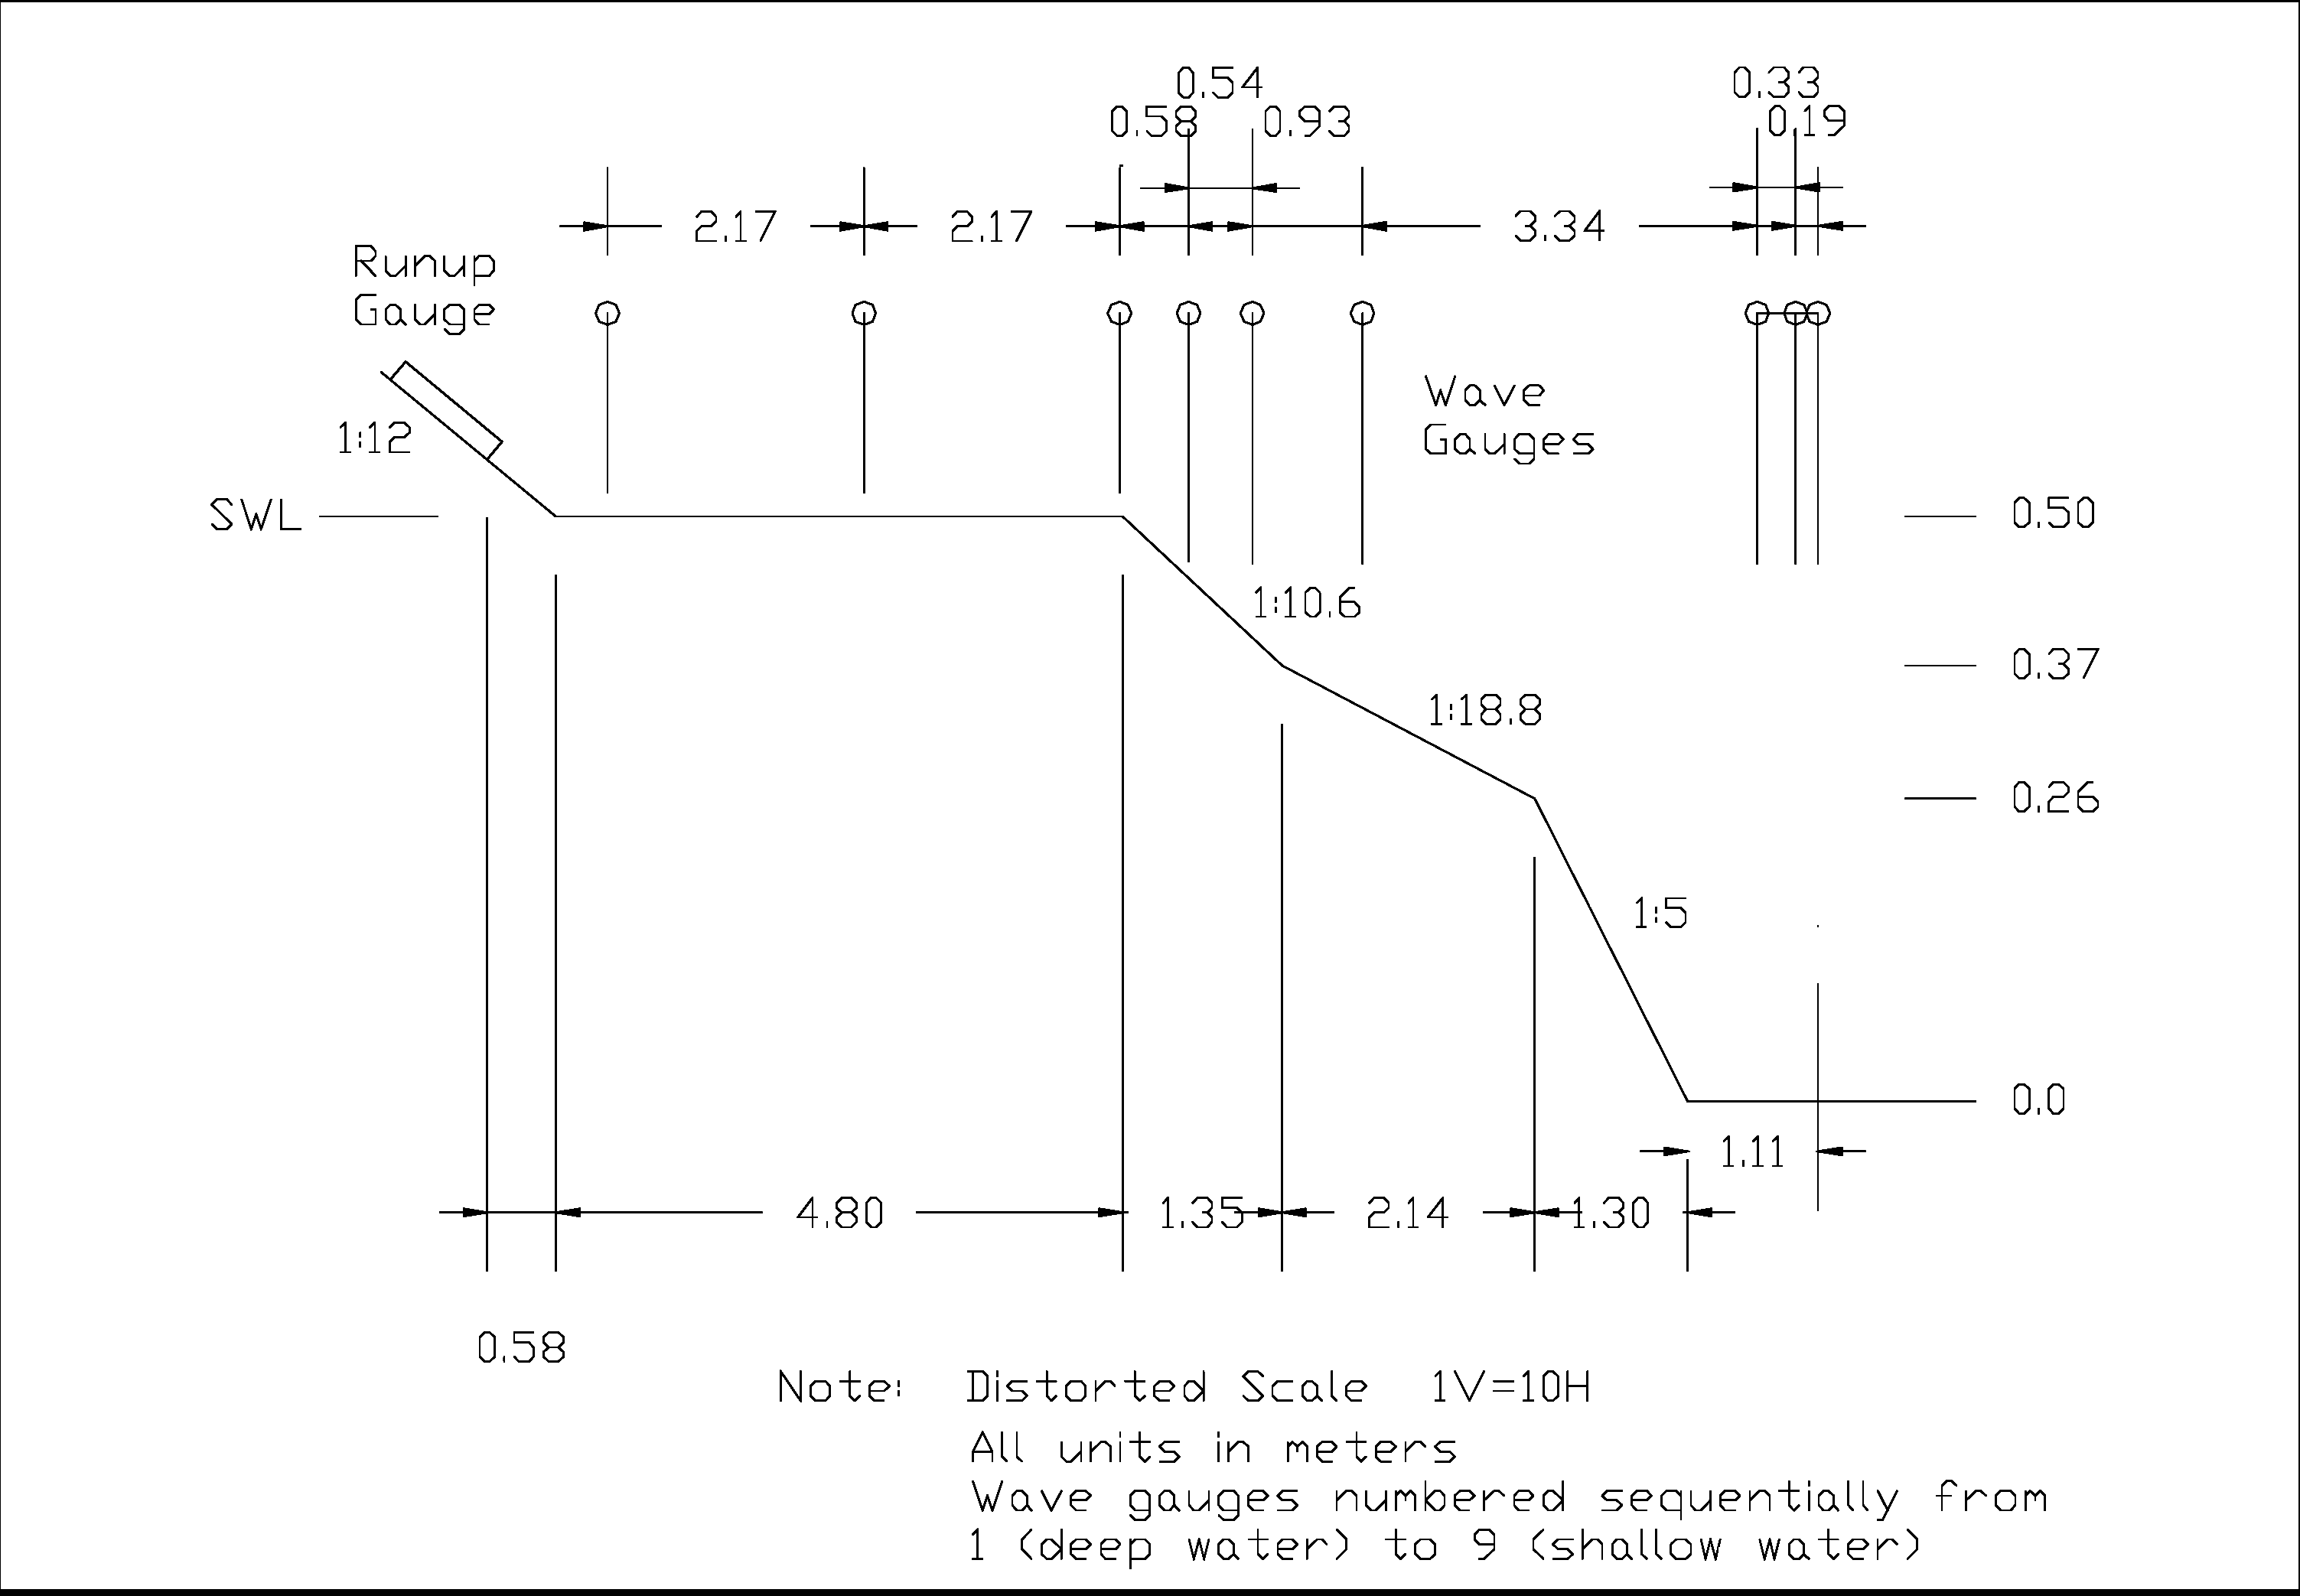
\includegraphics[scale=0.2]{./images/instrumen_eksperimen.png}
  \end{center}
  \caption{}
\end{figure}
\FloatBarrier

Ada 9 sensor gelombang dipasang disepanjang tabung eksperimen dengan jarak yang bervariasi, 2 sensor kecepatan angin, dan 1 sensor \emph{runup} gelombang. Wilayah penyebaran sensor gelombang dikelompokan menjadi 2. Wilayah pertama berada di atas karang dan wilayah kedua berada di laut. Wilayah yang lebih dalam dengan kedalaman yang konstan \cite{DemirbilekReport}. Wilayah karang merupakan gabungan dari wilayah karang yang datar \emph{Reef Flat} dan wilayah karang yang miring. Wilayah karang datar memiliki panjang mulai dari \emph{SWL} hingga 4.8 meter ke arah laut. Wilayah karang yang miring \emph{Reef Slope} di mulai dari bibir karang datar hingga 4.79 meter ke arah laut. Laut didefinisikan dengan wilayah dengan dasar terdalam. Sensor 1, 2, dan 3 tersebar di wilayah laut. Sensor 4, 5, dan 6 tersebar di wilayah \emph{reef slope}. Sensor 7, 8, dan 9 tersebar di wilayah \emph{reef flat}.

\subsection{Hasil Analisa Data}
    \begin{table}
    \begin{center}
      \begin{tabular}{|l|l|l|l|l|l|l|l|}
      \hline
      TestId & H & T & WL & $R_{max}$ & Wind \\ \hline
      Test99 & 5.5 & 1.25 & 50.0 & 1.5 & 7.1 \\ \hline
      Test100 & 6.0 & 1.0 & 50.0 & 1.6 & 6.9 \\ \hline
      Test101 & 3.3 & 1.0 & 50.0 & 0.7 & 5.3 \\ \hline
      Test102 & 8.2 & 2.5 & 53.1 & 8.4 & 7.0 \\ \hline
      Test103 & 8.6 & 2.0 & 53.1 & 7.8 & 7.1 \\ \hline
      Test104 & 8.0 & 1.75 & 53.1 & 6.7 & 5.8 \\ \hline
      Test105 & 7.8 & 1.5 & 53.1 & 5.9 & 6.3 \\ \hline
      Test106 & 5.4 & 1.5 & 53.1 & 4.0 & 6.7 \\ \hline
      Test107 & 6.3 & 1.25 & 53.1 & 4.5 & 6.8 \\ \hline
      Test108 & 6.6 & 1.0 & 53.1 & 6.4 & 6.7 \\ \hline
      Test109 & 3.8 & 1.0 & 53.1 & 5.3 & 6.5 \\ \hline
      \end{tabular}
      \end{center}
    \caption{Sampel data hasil analisa.}
    \end{table}
  \FloatBarrier
  Dari laporan \emph{"Laboratory Study of Wind Effect on Runup over Fringing Reefs"} \cite{DemirbilekReport} data yang di hasilkan berupa data hasil analisa yang berasal dari raw data yang merupakan time series. Pada table tersebut $H$ merupakan tinggi gelombang, $T$ merupakan spectral peak periods, $WL$ merupakan Wave Length, dan $R_{max}$ adalah ketinggian maksimum dari \emph{runup}. $H$, $WL$, dan $R_{max}$ merupakan dalam $cm$.

\section{Flowchart Sistem}

Secara keseluruhan, terdapat bentuk hirarki dalam sistem ini. Hirarki \emph{root} (Hirarki Utama), yakni sistem itu sendiri, bertugas sebagai pengatur. \emph{Root} memiliki anak yang memiliki tugas-tugas tertentu, seperti: $Membaca File$, $Transformasi Data$, $Membagi Data$, atau yang paling penting yakni $Training Data$.

\begin{figure}[ht]
  \caption{Flowchart Sistem}
  \begin{center}
    \tikzstyle{decision} = [diamond, draw, 
        text width=4.5em, text badly centered, node distance=3cm, inner sep=0pt]
    \tikzstyle{block} = [rectangle, draw, 
        text width=10em, text centered, rounded corners, minimum height=6em]
    \tikzstyle{blockTraining} = [rectangle, draw, fill=red!20, 
        text width=10em, text centered, rounded corners, minimum height=6em]
    \tikzstyle{line} = [draw, -latex']
    \tikzstyle{cloud} = [draw, ellipse,fill=red!20, node distance=3cm,
        minimum height=2em]
        
    \begin{tikzpicture}[node distance = 3cm, auto]
        % Place nodes
        \node [block] (init) {Mulai};
        \node [block, below of=init] (bacaData) {Membaca data report dari csv file};
        \node [block, below of=bacaData] (transformasiData) {Transformasi data menjadi matrix};
        \node [block, below of=transformasiData] (splitTrainingTesting) {Split data 80 persen training, 20 persen \emph{testing}};
        \node [block, below of=splitTrainingTesting] (setupEpochLr) {Menentukan jumlah epoch dan learning rate};
        \node [blockTraining, below of=setupEpochLr] (training) {Training Data};
        \node [blockTraining, below of=training] (testing) {Testing};
        \node [block, below of=testing] (stop) {Stop};
      
        % Draw edges
        \path [line] (init) -- (bacaData);
        \path [line] (bacaData) -- (transformasiData);
        \path [line] (transformasiData) -- (splitTrainingTesting);
        \path [line] (splitTrainingTesting) -- (setupEpochLr);
        \path [line] (setupEpochLr) -- (training);
        \path [line] (training) -- (testing);
        \path [line] (testing) -- (stop);
        \label{fig:sistem}
    \end{tikzpicture}
  \end{center}
\end{figure}
\FloatBarrier

\subsection{Flowchart Training}
Pada bagian training dan testing \ref{fig:sistem}, algoritma yang digunakan adalah algoritma ANN. Untuk testing, hanya dilakukan algoritma Feed Forward.
\begin{figure}[ht]
  \caption{Flowchart Training}
  \begin{center}
    \tikzstyle{block} = [rectangle, draw, fill=blue!20, 
        text width=10em, text centered, rounded corners, minimum height=6em]
    \tikzstyle{blockTraining} = [rectangle, draw, fill=red!20, 
        text width=14em, text centered, rounded corners, minimum height=2em]
    \tikzstyle{stopTrainng} = [rectangle, draw, fill=red!20, 
        text width=3em, text centered, rounded corners,  distance=10cm]
    \tikzstyle{line} = [draw, -latex']
    \tikzstyle{cloud} = [draw, ellipse,fill=red!20, node distance=2.3cm,
        minimum height=2em]
    \tikzstyle{decision} = [diamond, draw, fill=blue!20, 
        text width=4em, text badly centered, node distance=2.5cm, inner sep=0pt]
        
    \begin{tikzpicture}[node distance = 2cm, auto]
        % Place nodes
        \node [blockTraining] (init) {Mulai};
        \node [blockTraining, below of=init] (randomWeight) {Inisialisasi $weight$ dengan random data};
        \node [blockTraining, below of=randomWeight] (IW){Mengalikan Input Layer Dengan $Weight$ hidden layer};
        \node [blockTraining, below of=IW] (aktivasi){Jalankan fungsi aktivasi hidden layer};
        \node [blockTraining, below of=aktivasi] (HW){Mengalikan Input Layer Dengan $Weight$ untuk $output$};
        \node [blockTraining, below of=HW] (aktivasiOutput){Menjalankan fungsi aktivasi untuk output neuron};
        \node [blockTraining, below of=aktivasiOutput] (cost){Kalkulasi Error};
        \node [blockTraining, below of=cost] (stop){Stop};
  
        % Draw edges
        \path [line] (init) -- (randomWeight);
        \path [line] (randomWeight) -- (IW);
        \path [line] (IW) -- (aktivasi);
        \path [line] (aktivasi) -- (HW);
        \path [line] (HW) -- (aktivasiOutput);
        \path [line] (aktivasiOutput) -- (cost);
        \path [line] (cost) -- (stop);
    \end{tikzpicture}
  \end{center}
\end{figure}
\FloatBarrier
